\chapter{INTRODUÇÃO}

% Introdução ao assunto
\par 
Desde a descoberta da atividade el\'etrica do c\'erebro  e da inven\c{c}\~ao do \linebreak \ac{EEG}, por Hans Berger em 1924, foram desenvolvidas v\'arias id\'eias de como explorar esse acesso \`a fonte de pensamentos, emo\c{c}\~oes e a\c{c}\~oes humanas \cite{10.3389/fnins.2016.00530}.
\ac{BCIs} s\~ao dispositivos que se comunicam diretamente com os sinais cerebrais e permitem a intera\c{c}\~ao direta entre com o meio ambiente \cite{Rao2010}.
\par 
Inicialmente esse campo foi desenvolvido com um foco na restaura\c{c}\~ao de sentidos e mobilidade de pacientes, hoje em dia tamb\'em existe pesquisa em aplica\c{c}\~oes n\~ao-m\'edicas. Por exemplo, como um meio para verificar o alertid\~ao do usu\'ario executando um processo cri\'tico, um dispositivo para jogos e amplifica\c{c}\~ao f\'isica atrav\'es de exoesqueletos \cite{RAO}\cite{10.3389/fnins.2016.00530}.
\par
Para tanto o objetivo de uma \acs{BCI} \'e identificar e prever mudan\c{c}as induzidas pelo comportamento ou o estado cognitivo no sinal cerebral do usu\'ario \cite{Rao2010}.
\par
Para o desenvolvimento de uma \acs{BCI} normalmente s\~ao implementadas as seguintes etapas, como visto na figura \ref{fig:introduction} \cite{RAO}:
\begin{enumerate}
	\item \textbf{Capta\c{c}\~ao do Sinal cerebral}: Sinais cerebrais podem ser captados usando t\'ecnicas invasivas, semi-invasivas ou n\~ao-invasivas.
	
	\item \textbf{Processamento do Sinal}: Sinais brutos s\~ao processados apo\'s a aquisi\c{c}\~ao e t\'ecnicas de redu\c{c}\~ao de artefatos e extra\c{c}\~ao de caracter\'isticas s\~ao utilizadas.
	
	\item \textbf{Aprendizagem de maquina}: Neste est\'agio se gera o sinal de controle normalmente utilizando-se de algoritmos de aprendizagem de m\'aquina. 
	
	\item \textbf{Feedback sensorial}: O sinal de controle gera uma mudan\c{c}a no ambiente.
	Alguns desses mudan\c{c}as podem ser vistas, ouvidas ou sentidas pelo usu\'ario.
	
	\item \textbf{Processamento de sinais para a estimula\c{c}\~ao}: Antes de estimular uma regi\~ao particular no c\'erebro \'e importante sintetizar um padr\~ao de atividade que assemelha a atividade normalmente associada \`aquela regi\~ao. 
	\item \textbf{Estimula\c{c}\~ao cerebral}: O padr\~ao de estimula\c{c}\~ao da etapa anterior \'e utilizada em conjunto com uma t\'ecnica de estimula\c{c}\~ao invasiva ou n\~ao-invasiva para estimular o c\'erebro. 
\end{enumerate}
\par
Durante o desenvolvimento de interfaces cerebrais n\~ao-invasivas utilizando-se do \ac{EEG} encontram-se dois obst\'aculos principais: O fato do sinal ser n\~ao estacion\'ario e sua variabilidade inerente \cite{Rao2010}.
Dados do mesmo paradigma experimental mas de sess\~oes diferentes provavelmente exibir\~ao diferen\c{c}as devido a, por exemplo, ligeiras mudan\c{c}as nas posi\c{c}\~oes dos eletrodos ou mudan\c{c}as nas propriedades eletromec\^anicas eletrodos tal como sua imped\^ancia \cite{Rao2010}.
Al\'em disto, a superposi\c{c}\~ao ruidosa e n\~ao linear da atividade das popula\c{c}\~oes medidas no couro cabeludo podem mascarar os padr\~oes neurais e dificultar sua detec\c{c}\~ao \cite{Rao2010}.
Devido a esses fatores, t\'ecnicas de processamento de sinal estat\'isticas e de aprendizagem de maquina tem uma import\^ancia fundamental durante o processo de reconhecimento de padr\~oes \ac{EEG} e traduzi-los para um sinal de controle \cite{Rao2010}.

\begin{figure}[h!]
	\label{fig:introduction}
	\caption{Est\'agios de uma interface cerebral \cite{Rao2010}}
	\centering
	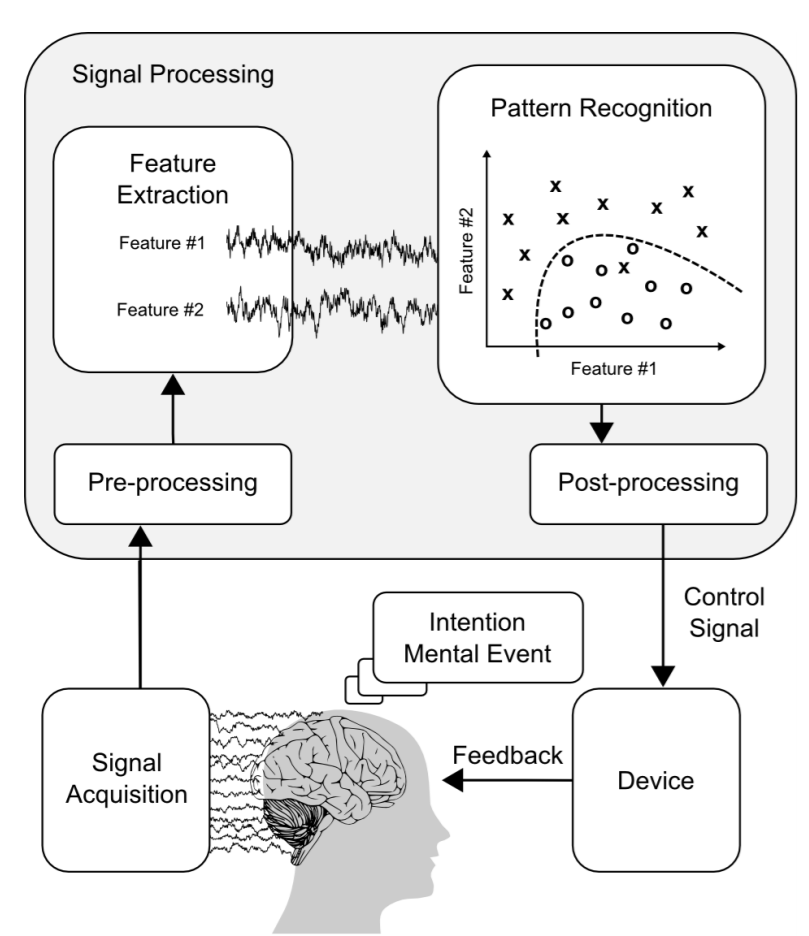
\includegraphics[scale=0.45]{./figuras/bci-stages}
\end{figure}

\section{Objetivo}
%Objetivo Principal
O objetivo principal deste  \ac{TCC} \'e realizar a comparação de m\'etodos de aprendizagem de m\'aquina e processamento de sinais cerebrais para melhor entender como estes fatores afetam a qualidade da classifica\c{c}\~ao permitindo o desenvolvimento de uma \acs{BCI} mais precisa.
\par 
Considerando estes fatores neste trabalho foram explorados e comparados m\'etodos de aprendizagem de m\'aquina tais como redes neurais e SVMs (kernel linear e gaussiano). Tamb\'em foram comparados m\'etodos estimativa de espectro (PMTM, Welch e periodograma) com diferentes configura\c{c}\~oes de comprimento e sobreposi\c{c}\~ao entre as janelas amostradas.
%Objetivo Secundários
Para fazer isto foi nescess\'ario obter as amostras de eletroencefalograma para a classifica\c{c}\~ao;
desenvolver o framework para realizar as compara\c{c}\~oes; fazer a an\'alise dos resultados.
%quatro objetivos secundarios

